\documentclass[11pt]{article}

\usepackage[utf8]{inputenc}
\usepackage[portuges]{babel}
\usepackage{indentfirst}
\usepackage{natbib}
\usepackage{graphicx}
\usepackage{geometry}
\usepackage[export]{adjustbox}
\usepackage[shortlabels]{enumitem}
\usepackage{minted}
\usepackage{makeidx}
\usepackage{newfloat}
\usepackage{lipsum}
\usepackage{enumitem}
\usepackage{multirow}
\usepackage{array}
\usepackage{underscore}

 \geometry{
    a4paper,
    total={130mm,227mm},
    left=40mm,
    top=40mm,
}
\addto\captionsportuges{
    \renewcommand*\contentsname{\LARGE Índice}}

\begin{document}

\begin{titlepage}
    \begin{center}
        
\includegraphics[width=0.4\textwidth]{Imagens/uni.png}
    
        \vspace{2cm}
        
        \textbf{\Huge Laboratórios de Informática III}\par

        \vspace{3cm}
        
        \large \\
        
        Carlos Diogo Fernandes Pina A95349 \\
        Lara Beatriz Pinto Ferreira A95454 \\ 
        João Machado Gonçalves A97321 \\

        \vspace{2cm}
    
        \begin{figure}[hbt!]
        \minipage{0.3\textwidth}
            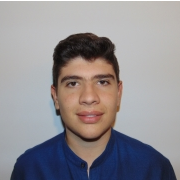
\includegraphics[width=\linewidth]{Imagens/febras.png}
            \centering
            \captionsetup{A95349}
        \endminipage\hfill
        \minipage{0.3\textwidth}
            
\includegraphics[width=\linewidth]{Imagens/Photo (2).jpg}
            \centering
            \captionsetup{A95454}
        \endminipage\hfill        
        \minipage{0.3\textwidth}
            
\includegraphics[width=\linewidth]{Imagens/slash.png}
            \centering
            \captionsetup{A97321}
        \endminipage
        \end{figure}
        
        \vspace{3cm}
        \textbf{18 de Novembro de 2023}
    \end{center}
    

\end{titlepage}


\thispagestyle{empty}
\cleardoublepage
\tableofcontents 
\clearpage


\section {Introdução}
    No âmbito da Unidade Curricular de Laboratórios de Informática III da licenciatura em Engenharia Informática, nesta primeira fase de avaliação, foi nos requisitado a implementação de um \textit{parser} em C que validasse as linhas dos quatro ficheiros \textit{.csv} (\textit{users}, \textit{flights}, \textit{passengers} e \textit{reservations}) que nos foram disponibilizados.
    Foi-nos também solicitado a implementação de pelo menos seis \textit{queries}, que no caso resolvermos implementar as \textit{queries 1,3,4,5,8,9}.
    
\section{Estratégia utilizada}
    Após a leitura do enunciado optamos por criar catálogos para as \textit{structs} \textit{users}, \textit{flights}, \textit{reservations} e \textit{passengers}, e percorrê-los de forma iterativa.
    \subsection{Estruturas de dados utilizadas para representar utilizadores, voos, reservas e passageiros}
    As estruturas de dados referidas foram criadas de forma a ser possível realizar, o mais eficientemente possível, tanto a nível de performance como de memória, as \textit{queries} que implementamos.
    
\subsubsection{Utilizadores}
    Utilizamos depois um catálogo \textit{users} construido com base na \textit{struct users} com o objetivo de conseguirmos encontrar e manipular, de modo eficiente, informações sobre um certo \textit{user}, através do seu \textit{ID}, que é a \textit{key} da \textit{hashtable}. Deste modo, decidimos armazenar a informação dos \textit{users} através do uso de \textit{hashtables}, pois achamos que é a maneira mais eficiente de implementar o objetivo descrito.
    
    \begin{figure}[hbt!]
        \centering
        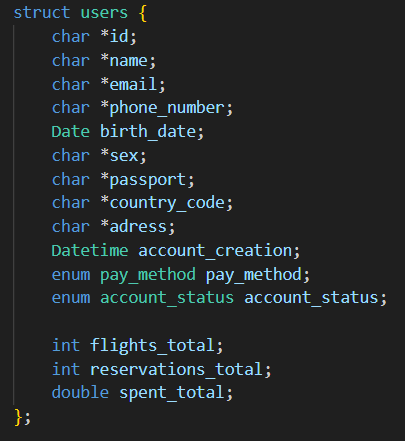
\includegraphics[width=0.5\textwidth]{users.png}
        \caption{Struct Users}
        \label{fig:example}
    \end{figure}
    \newpage
     \begin{itemize}
                \item Id : O identificador do \textit{user} é representado como uma \textit{string}
                \item Name : O Nome do \textit{user} é representado como uma \textit{string}
                \item Email : O email do \textit{user} é representado como uma \textit{string}
                \item Phone_number : O número de telemóvel do \textit{user} é representado como uma \textit{string}
                \item Birth_date : A data de nascimento do \textit{user} é representada como um \textit{datetime}
                \item Sex : O género do \textit{user} é representado como uma \textit{string}
                \item Passaport : O númerop do passaporte do \textit{user} é presentado como uma \textit{string}
                \item Country_code : O código do país de residência
                \item Address : A morada do \textit{user} é representado como uma \textit{string}
                \item Account_creation : A data de criação da conta é representada com um \textit{datetime}
                \item Pay_method : O método de pagamento é representado como um \textit{enum} 
                \item Account_status : O estado da conta é representado como um \textit{enum} 
                \item Flights_total : O número de voos realizados pelo \textit{user} é representado como um inteiro
                \item Reservations_total : O número de reservas realizadas pelo \textit{user} é representado como um inteiro
                \item Spent_total : O total de dinheiro gasto pelo \textit{user} é representado como um \textit{double}
        \end{itemize}
\newpage
\subsubsection{Voos}
    Utilizamos depois um catálogo \textit{flights} construido
    com base na \textit{struct flights} com o objetivo de conseguirmos encontrar e manipular, de modo eficiente, informações sobre um certo \textit{flight}, através do seu \textit{ID}, que é a \textit{key} da \textit{hashtable}. Deste modo, decidimos armazenar a informação dos \textit{flights} através do uso de \textit{hashtables}, pois achamos que é a maneira mais eficiente de implementar o objetivo descrito.

    \begin{figure}[hbt!]
        \centering
        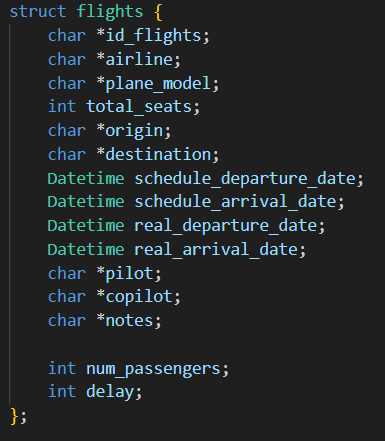
\includegraphics[width=0.5\textwidth]{flights.png}
        \caption{Struct Flights}
        \label{fig:example}
    \end{figure}
    
     \begin{itemize}
        \item Id_flights : O identificador do \textit{Flight} é representado como uma \textit{string}
        \item Airline : A companhia aérea que realizou o \textit{Flight} é representada com uma \textit{string}
        \item Plane_model : O modelo do avião usado na \textit{Flight} é representada com uma \textit{string}
        \item Total_seats: O número de lugares total do avião usado na \textit{Flight} é representada como um inteiro
        \item Origin : O aeroporto de origem da \textit{Flight} é representada como uma \textit{string}
        \item Destination : O aeroporto de destino da \textit{Flight} é representada como uma \textit{string}
        \item Schedule_departure_date : A data e hora planeada para a partida da \textit{Flight} é representado por um \textit{datetime}
        \item Schedule_arrival_date :  A data e hora planeada para a chegada da \textit{Flight} é representado por um \textit{datetime}
        \item Real_departure_date : A data e hora efetiva da partida da \textit{Flight} é representado por um \textit{datetime} 
        \item Real_arrival_date : A data e hora efetiva da \textit{Flight} é representado por um \textit{datetime} 
        \item Pilot : O nomedo  piloto que realizou a \textit{Flight} é representado por uma \textit{string}
        \item Copilot : O nome do Co-piloto que realizou a \textit{Flight} é representado por uma \textit{string}
        \item Notes : As observações sobre a \textit{Flight} são representadas como uma \textit{string}
        \item num_passengers : O número de passageiros que realizou a \textit{Flight} é representado como um inteiro
        \item Delay : O atraso da \textit{flight}, em segundos, é representado como um inteiro
    \end{itemize}
\subsubsection{Reservas}
    Utilizamos depois um catálogo \textit{reservations} construido
    com base na \textbf{struct reservations} com o objetivo de conseguirmos encontrar e manipular, de modo eficiente, informações sobre um certo \textit{reservation}, através do seu \textit{ID}, que é a \textit{key} da \textit{hashtable}. Deste modo, decidimos armazenar a informação dos flights através do uso de \textit{hashtables}, pois achamos que é a maneira mais eficiente de implementar o objetivo descrito.
    
    \begin{figure}[hbt!]
        \centering
        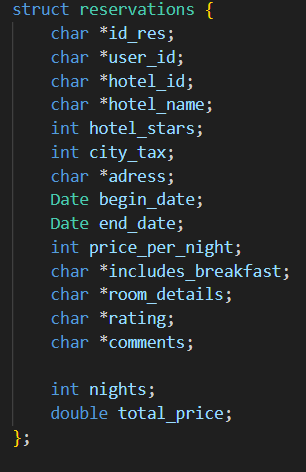
\includegraphics[width=0.4\textwidth]{reservations.png}
        \caption{Struct Reservations}
        \label{fig:example}
    \end{figure}
    
    \newpage
    
     \begin{itemize}
        \item Id_res : O identificador da \textit{Reservation} é representado como uma \textit{string}
        \item User_id : O identificador do \textit{User} que fez a \textit{Reservation} é representado como uma \textit{string}
        \item Hotel_id : O identificador do hotel é representado como uma \textit{string}
        \item Hotel_name : O nome do hotel é representado como uma \textit{string}
        \item Hotel_stars : O número de estrelas do hotel é representado como um inteiro
        \item City_tax : A percentagem do imposto da cidade é representado como um inteiro
        \item Begin_date : A data de início da \textit{Reservation} é representado como uma \textit{date}
        \item End_date : A data de fim da \textit{Reservation} é representado como uma \textit{date}
        \item Price_per_night : O preço por noite é representado por um inteiro
        \item Includes_breakfast : A inclusão de pequeno-almoço na \textit{Reservation} é representa como uma \textit{string}
        \item Room_details : Os detalhes sobre o quarto são representado como uma \textit{string} 
        \item Rating : A classificação atribuída pelo \textit{user} é representada como uma \textit{string}
        \item Comment : O comentário sobre a reserva 
        \item Nights : O número de noites que abrangidas na \textit{Reservation} é representada como um inteiro
        \item Total_price : O preço total da \textit{Reservation} é representado como um \textit{double}
    \end{itemize}
\newpage
\subsubsection{Passageiros}
    Utilizamos depois um catálogo \textit{passengers} construido
    com base na \textit{struct passengers} com o objetivo de conseguirmos encontrar e manipular, de modo eficiente, informações sobre um certo \textit{passenger}, através do \textit{ID} do \textit{Flight}, que é a \textit{key} da \textit{hashtable}. Deste modo, decidimos armazenar a informação dos \textit{flights} através do uso de \textit{hashtables}, pois achamos que é a maneira mais eficiente de implementar o objetivo descrito.
    
    \begin{figure}[hbt!]
        \centering
        \includegraphics[width=0.6\textwidth]{Captura de ecrã 2023-11-22 224328.png}
        \caption{Struct Passengers}
        \label{fig:example}
    \end{figure}
    
    \begin{itemize}
        \item Flight_Id : O identificador da \textit{Flight} é representado como uma \textit{string}
        \item User_Id : O identificador do \textit{User} é representado como uma \textit{string}
    \end{itemize}
\newpage


\subsection{Estratégia de modularização e reutilização de código}
A modularização e reutilização do código, apesar de não serem avaliados nesta fase, promovem uma maior organização, leitura e facilidade de manutenção do código, que por sua vez auxiliam no processo de desenvolvimento, desta forma decidimos implementar os seguintes módulos:
    \begin{itemize}
        \item Users : Representação de um \textit{User} e catalogo dos mesmos
        \item Flights : Representação de um \textit{Flight} e catalogo dos mesmos
        \item Reservations : Representação de um \textit{Reservation} e catalogo dos mesmos
        \item Passengers : Representação de um \textit{Passenger} e catalogo dos mesmos
        \item Catalog : Agregação dos diversos catalogos e estruturas
        \item Date : Representação de um \textit{Date} e/ou \textit{Datetime}
        \item Valid : Agregado de métodos de validação 
    \end{itemize}

\subsection{Estratégia de encapsulamento e abstração}
De forma a manter o código seguro e bem estruturado, todos os módulos escondem a sua implementação de maneira que toda a operação sobre os seus dados pode ser feita com as funções que estes disponibilizam.

\newpage

\section{Queries}
Com os dados já validados e organizados, foi nos pedido o processamento dos mesmo usando diferentes queries, estas suportam também a flag 'F', isto é, uma query com esta flag apresenta o seu resultado no output no formato \textit{field: value}.

\subsection{Query 1}
\subsubsection{Descrição}
\textbf{Q1}: Listar o resumo de um utilizador, voo, ou reserva, consoante o identificador recebido por argumento. É garantido que não existem identificadores repetidos entre as diferentes entidades. A query deverá retornar as seguintes informações:
    \begin{itemize}
        \item Utilizador: nome;sexo;idade;código_do_país;passaporte;número_voos;número_reservas;total_gasto(name;sex;age;country_code;number_of_flights;number_of_reservations;total_spent)
        \item Voo:
companhia;avião;origem;destino;partida_est;chegada_est;número_passageiros;tempo_atraso(airline;plane_model;origin;destination;schedule_departure_date;schedule_arrival_date;passengers;delay)
        \item Reserva:
id_hotel;nome_hotel;estrelas_hotel;data_início;data_fim;pequeno_almoço;número_de_noites;preço_total(hotel_id;hotel_name;hotel_stars;begin_date;end_date;includes_breakfast;nights;total_price)
    \end{itemize}

    \begin{figure}[hbt!]
    \centering
    \includegraphics[width=0.6\textwidth]{comandq1.png}
    \caption{Comando Query 1}
    \label{fig:example}
\end{figure}
    
\subsubsection{Implementação}
Se o identificador conter apenas dígitos, procuramos na hashtable das \textit{flights}, caso contrário, se os primeiros 4 caracteres forem '\textit{Book}', procuramos na hashtable das \textit{reservations}, caso nenhuma das condições anteriores se verifique, pesquisamos na hashtable dos \textit{users}.
Em todos os casos é devolvida uma cópia dos valores encontrados ou nada se não existirem exceto no caso dos utilizadores com \textit{account_status = “inactive”} que também não devolve nada.

\newpage
\subsection{Query 3}
\textbf{Q3}: Apresentar a classificação média de um hotel, a partir do seu identificador.

\begin{figure}[hbt!]
    \centering
    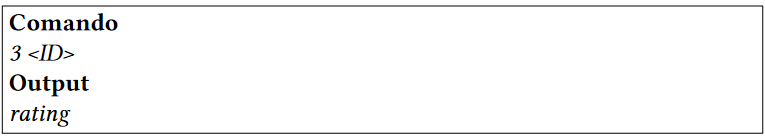
\includegraphics[width=0.6\textwidth]{comandq3.png}
    \caption{Comando Query 3}
    \label{fig:example}
\end{figure}

\subsubsection{Implementação}
Procuramos todas as \textit{reservations}, na hashtable das mesmas, que foram efetuadas no hotel com o identificador especificado e obtemos todas classificações. No fim, calculamos a media dessas classificações.

\subsection{Query 4}
\textbf{Q4}: Listar as reservas de um hotel, ordenadas por data de início (da mais recente para a mais
antiga). Caso duas reservas tenham a mesma data, deve ser usado o identificador da reserva como critério de desempate (de forma crescente)

\begin{figure}[hbt!]
    \centering
    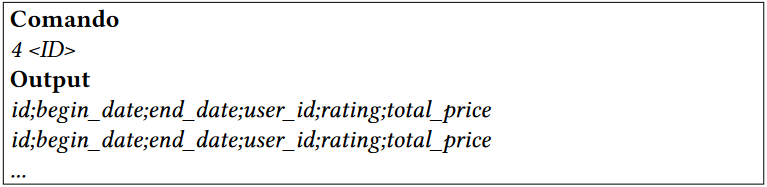
\includegraphics[width=0.6\textwidth]{comandq4.png}
    \caption{Comando Query 4}
    \label{fig:example}
\end{figure}

\subsubsection{Implementação}
Procuramos todas as \textit{reservations}, na hashtable das mesmas, as que foram efetuadas no hotel com o identificador especificado e usamos-las para criar uma lista, de seguida organizamos essa mesma lista consoante os requisitos em cima.

\newpage
\subsection{Query 5}
\textbf{Q5}: Listar os voos com origem num dado aeroporto, entre duas datas, ordenados por data de partida
estimada (da mais antiga para a mais recente). Um voo está entre <begin_date> e <end_date> caso a
sua respetiva data estimada de partida esteja entre <begin_date> e <end_date> (ambos inclusivos).
Caso dois voos tenham a mesma data, o identificador do voo deverá ser usado como critério de
desempate (de forma crescente).

\begin{figure}[hbt!]
    \centering
    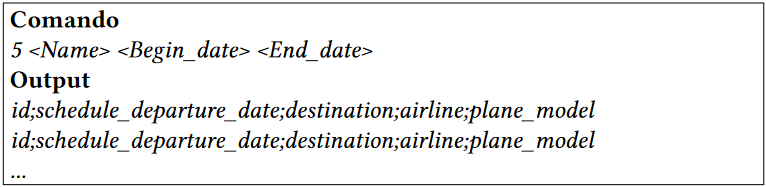
\includegraphics[width=0.6\textwidth]{comandq5.png}
    \caption{Comando Query 5}
    \label{fig:example}
\end{figure}

\subsubsection{Implementação}
Procuramos todas as \textit{flights}, na \textit{hashtable} das mesmas, que foram efetuadas numa origem e período especificados e usamos-las para criar uma lista e organizamos essa mesma lista consoante os requisitos em cima.

\subsection{Query 8}
\textbf{Q8}: Apresentar a receita total de um hotel entre duas datas (inclusive), a partir do seu identificador. As receitas de um hotel devem considerar apenas o preço por noite (price_per_night) de todas as
reservas com noites entre as duas datas. E.g., caso um hotel tenha apenas uma reserva de 100€/noite de 2023/10/01 a 2023/10/10, e quisermos saber as receitas entre 2023/10/01 a 2023/10/02, deverá ser retornado 200€ (duas noites). Por outro lado, caso a reserva seja entre 2023/10/01 a 2023/09/02, deverá ser retornado 100€ (uma noite).

\begin{figure}[hbt!]
    \centering
    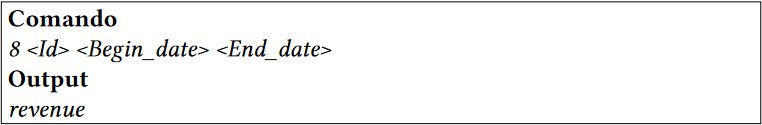
\includegraphics[width=0.6\textwidth]{comandq8.png}
    \caption{Comando Query 8}
    \label{fig:example}
\end{figure}

\subsubsection{Implementação}
Procuramos todas as \textit{reservations}, na \textit{hashtable} das mesmas, que foram efetuadas num hotel e período especificados, calculamos o preço de cada \textit{reservation} nesse período e somamos à receita total.


\newpage
\subsection{Query 9}


\textbf{Q9}: Listar todos os utilizadores cujo nome começa com o prefixo passado por argumento, ordenados
por nome (de forma crescente). Caso dois utilizadores tenham o mesmo nome, deverá ser usado
o seu identificador como critério de desempate (de forma crescente). Utilizadores inativos não
deverão ser considerados pela pesquisa.

\begin{figure}[hbt!]
    \centering
    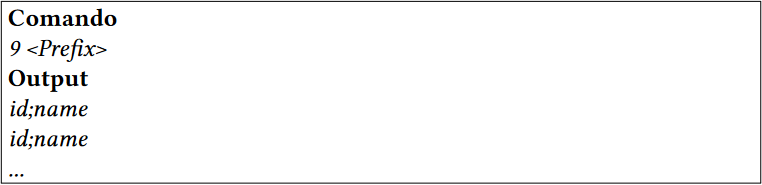
\includegraphics[width=0.6\textwidth]{comandq9.png}
    \caption{Comando Query 9}
    \label{fig:example}
\end{figure}

\subsubsection{Implementação}
Procuramos todas os \textit{users}, na \textit{hashtable} dos mesmos, cujo nome começa com o prefixo especificado e a sua conta não está inativa, usamos-los para criar uma lista e organizamos essa mesma lista consoante os requisitos em cima.


\section{Conclusão}
O trabalho desenvolvido nesta primeira fase satisfez, de uma forma geral, todos os requisitos presentes para esta fase. Este projeto foi desenvolvido com o objetivo de ser o mais eficiente e rápido possível, tentando sempre cumprir as regras de encapsulamento e modularidade. Embora exista sempre espaço para melhorar o trabalho, encontramos-nos satisfeitos com esta entrega.

\end{document}
